%\usepackage{textcomp}
\usepackage[utf8]{inputenc}
\usepackage{pifont}
\usepackage{arev}
%\graphicspath{{../../sems-media/priv/}}
%%%%%%%%%%%% Festlegung der Titelseite %%%%%%%%%%%%%%%%%%%%%%%%%%%%%%%%%

\author[
	\textbf{\href{http://www.sbi.uni-rostock.de/team/single/martin-peters/}{Martin Peters}}
]
{
	\underline{\textsc{\href{http://freakybytes.net}{Martin Peters}}}
}

%\date{\today} % Hier kann das Datum des Vortrages festgelegt werden (fuer Fusszeile etc.)
\date{2016-09-21}

\institute{%
{\scriptsize{%
%$^1$
Department of Systems Biology \& Bioinformatics, %\\
University of Rostock\\
\\[5em]
}}
%
%\textcolor{colorscheme}{\href{http://sems.uni-rostock.de}{http:\twobar{}sems.uni-rostock.de}\\[2.5em]}
%\vspace{1em}
}


\titlegraphic{
%\begin{minipage}[b]{13.5em}
%	\raisebox{-1.5px}{
\includegraphics[height=1em]{res/COMBINE.png}}
%	\ 2016
%\end{minipage}
%\begin{minipage}[t]{10em}
%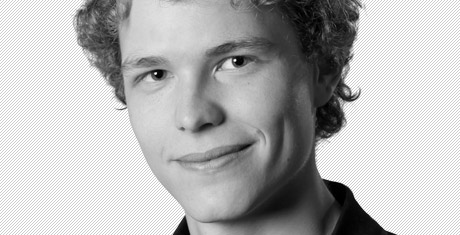
\includegraphics[width=10em]{peters.jpg}
%\end{minipage}
}
\title[Storage Solution for Models with Multiple Versions]{\Large Storage Solution for Models with Multiple Versions}
\subtitle{\small Concept and Prototype Implementation}


% ein alternatives Titelbild kann mittels 
%\titleimage{Dateiname.xyz}
% angegeben werden (auf vernuenftiges Seitenformat und Kontrastwerte achten, Skalierung und Abschneiden der oberen rechten Ecke passieren automatisch)
%\titleimage{scharm_02.jpg}
\titleimage{}
%%%%%%%%%%%% Festlegungen fuer Kopf- und Fusszeile %%%%%%%%%%%%%%%%%%%%
% Institutsname f\"ur die Fusszeile (nur wenn bei Paketeinbindung 'footuni' angegeben ist)
\footinstitute{Department of Systems Biology \& Bioinformatics\\Faculty of Computer Science \& Electrical Engineering}%Mathematisch-Naturwissenschaftliche Fakult\"at, Institut f\"ur Physik}
% eigenes Logo oben rechts hinzufuegen (bitte auf vernuenftiges Format achten - ein zu hohes Logo verschiebt das Layout)
\renewcommand{\mylogo}{
	%\hfill 
\includegraphics[height=8mm]{./unirostock/institutslogo}
	%\hfill 
\includegraphics[trim=22.2cm 0cm 0cm 8.6cm,clip=true,height=8mm]{./unirostock/sems_2}
}

\usepackage{listings}
\usepackage{tikz}
\usepackage{pgfplots}
\usetikzlibrary{shapes,arrows,trees,decorations.pathmorphing,backgrounds,fit}
 
\newcommand{\newsection}[1]{
\section{#1}
%\begin{frame}{#1}\tableofcontents[currentsection]\note{tof: #1}\end{frame}
}
\usepackage{tabularx}
\usepackage{wasysym}
\usepackage[misc]{ifsym}

\lstset{%
    %numbers=left,
    %numberstyle=\tiny\color{gray},
    %frame=tb
  }

% show other people's slides
\newenvironment{changemargin}[2]{%
\begin{list}{}{%
\setlength{\topsep}{0pt}%
\setlength{\leftmargin}{#1}%
\setlength{\rightmargin}{#2}%
\setlength{\listparindent}{\parindent}%
\setlength{\itemindent}{\parindent}%
\setlength{\parsep}{\parskip}%
}%
\item[]}{\end{list}}
\newcommand{\maxFrameImage}[2]{
\begin{frame}[plain]%
% \begin{tikzpicture}[overlay]%
% \draw[fill=red] (0,0) -- (-20,0) -- (-20,-20) -- (0,-20);%
% \end{tikzpicture}%
\begin{changemargin}{-1.45cm}{-1cm}
\begin{center}
\begin{tikzpicture}[overlay]
\fill[white] (-100,-100) rectangle (100,100);
\node[fill=white] (db4) at (0,-1) {\includegraphics[width=\paperwidth,height=\paperheight,keepaspectratio]{#1}};
\end{tikzpicture}
\end{center}#2
\end{changemargin}
\end{frame}
}

\usepackage{varwidth}

\definecolor{chck}{RGB}{0,155,85}


